\begin{document}
\section{Sensorer}
Kilde: \cite{tikNXT}
\subsection{Afstandssensorer}
\subsubsection{Ultrasonic}
Ultrasonic sensoren(US)(\ref{us}) er en sensor der kan måle afstande til objekter.

\begin{figure}[h]
\centering
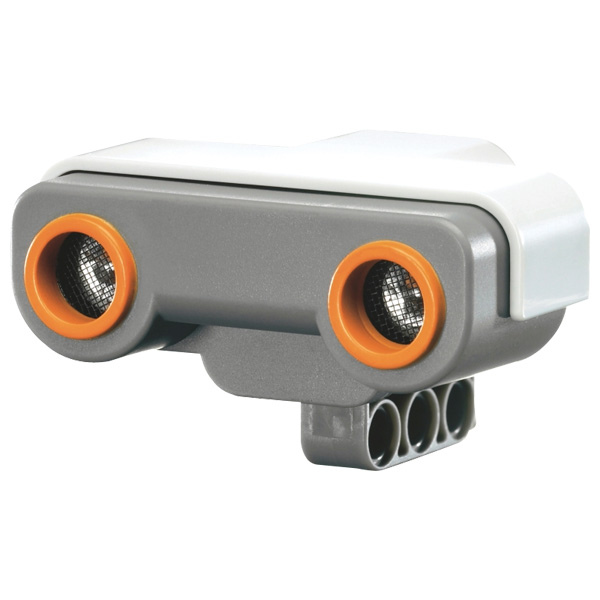
\includegraphics[width=10cm]{us}
\caption{Lego Mindstorms Ultrasonic Sensor}
\end{figure}

Dette gøres ved at der sendes en lydbølge og der så beregnes hvor lang tid det tager for denne at ramme objektet og så komme tilbage igen.
US'en måler afstanden i cm eller tommer og den maksimale aftsand der kan måles er 255 cm med en præcision på +-3 centimeter.
\\
\\
Eksperimenter\cite{tikNXT} har vist:
\begin{itemize}
\item Det har vist sig at den minimale aftsand der kan måles er 3 cm.
\item Desuden er det bedst genkendelig objekt et objekt der har glat og hård overflade og som er firkantet.
\item Desto mindre objektet er desto sværer har sensoren ved at se objektet.
\item Sensorens højre 'øje' er det der sender lydbølgen mens det venstre modtager.
Det gør at US'en 'ser' bedre i højre side når sensoren befinder sig i horisontal position.
Dette kan tydelig ses når afstand mellem sensor og objekt er under 20 cm, da den slet ikke kommer i sensorens synsfelt i venstre side.
\item Hvis sensoren anvendes i vertikal position er der det problem at modtagelsen af bølgerne kan blive distraheret af underlaget.
\end{itemize}

Den bedste opstilling for US'en er i horisontal position, der opnåes de bedste resultater fordi den kritiske region ifht. den vertikale position er mindre.
En vinkel på mere end 15 grader fra lydbølgen giver hellere ikke klare resultater, desuden er runde genstande også svært genkendelige for US'ens synsfelt.

\subsubsection{Test}
Der er gennemført en mindre test af US'en, for at svare på følgende spørgsmål:

\begin{itemize}
\item Hvor langt rækker US'en i praksis?
\item Hvor stor nøjagtighed har den i praksis?
\item Ligner resultaterne dem fra eksperimenterne ovenfor?
\end{itemize}

For at svare på disse spørgsmål kom vi frem til følgende forsøgsopstilling(\ref{opstilling}).

\begin{figure}[h]
\centering
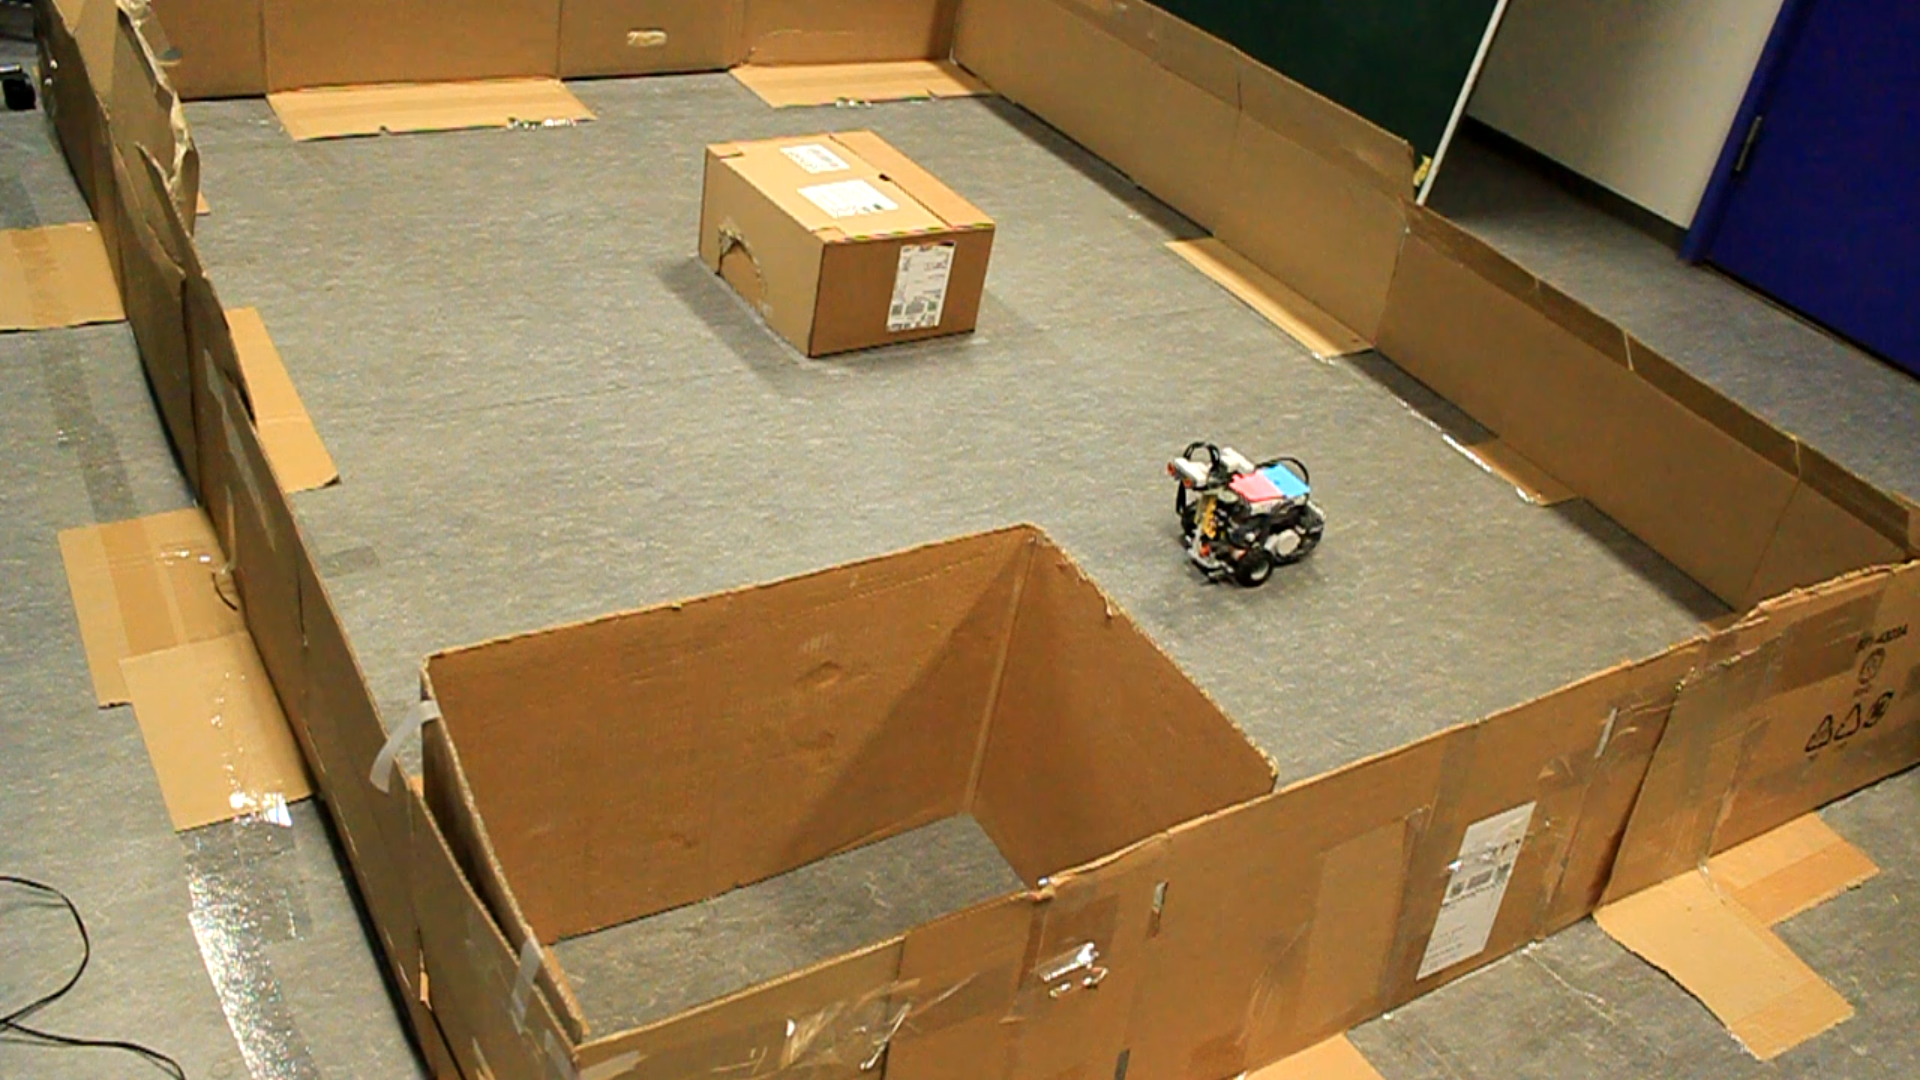
\includegraphics[width=10cm]{opstilling}
\caption{Forsøgsopstilling for test af US'ens afstands præcision}
\label{opstilling}
\end{figure}

Forsøgsopstillingen består af følgende dele:
\begin{itemize}
\item Tommestok
\item NXT v2
\item Lego Mindstorms Ultrasonic Sensor
\end{itemize}

Tommestokken blev brugt til at måle den nøjagtige afstand og derefter blev sensoren aflæst.
På \ref{us_data} kan man se de indsamlede data fra forsøget.
\bruno{skal evt. i appendix}

\begin{figure}[h]
\centering
\begin{tabular}{r | c | c | c |}
optimal & test1 & test2 & test3 \\
\hline
1 & 6 & 6 & 6 \\
10&	22&	23&	23\\
20&	22&	23&	23\\
30&	31&	31&	32\\
40&	40&	41&	40\\
50&	50&	50&	51\\
60&	60&	61&	61\\
70&	70&	71&	66\\
80&	80&	81&	81\\
90&	90&	91&	91\\
100&	100&	101&	102\\
110&	111&	112&	112\\
120&	120&	121&	121\\
130&	131&	131&	131\\
140&	141&	141&	141\\
150&	151&	151&	151\\
160&	161&	161&	163\\
170&	171&	171&	171\\
180&	255&	181&	181\\
190&	255&	190&	191\\
200&	202&	201&	202\\
210&	255&	255&	213\\
220&	255&	255&	222\\
230&	255&	255&	232\\
240&	255&	255&	255\\
250&	255&	255&	255\\
260&	255&	255&	255\\
\end{tabular}
\caption{Forsøgsresultater: afstande til objekt i cm.}
\label{us_data}
\end{figure}

På figur \ref{us_diagram} kan det ses hvordan at de tre tests alle giver forkerte resultater når US'en er mindre en 20 cm fra objektet.
Desuden kan det ses på \ref{us_diagram} at der i test1 kun kunne måles op til 170 cm før der opstod usikkerhed, men de andre tests nåede 200(test2) og 230(test3) cm før der opstod størrer usikkerhed.
Generelt holder det som der bliver lovet, nemlig at der er en afvigelse på 3 cm på målingerne, men forsøget viser at der kun med sikkerhed kan måles mellem 20 og 170 cm.

\begin{figure}[h]
\centering
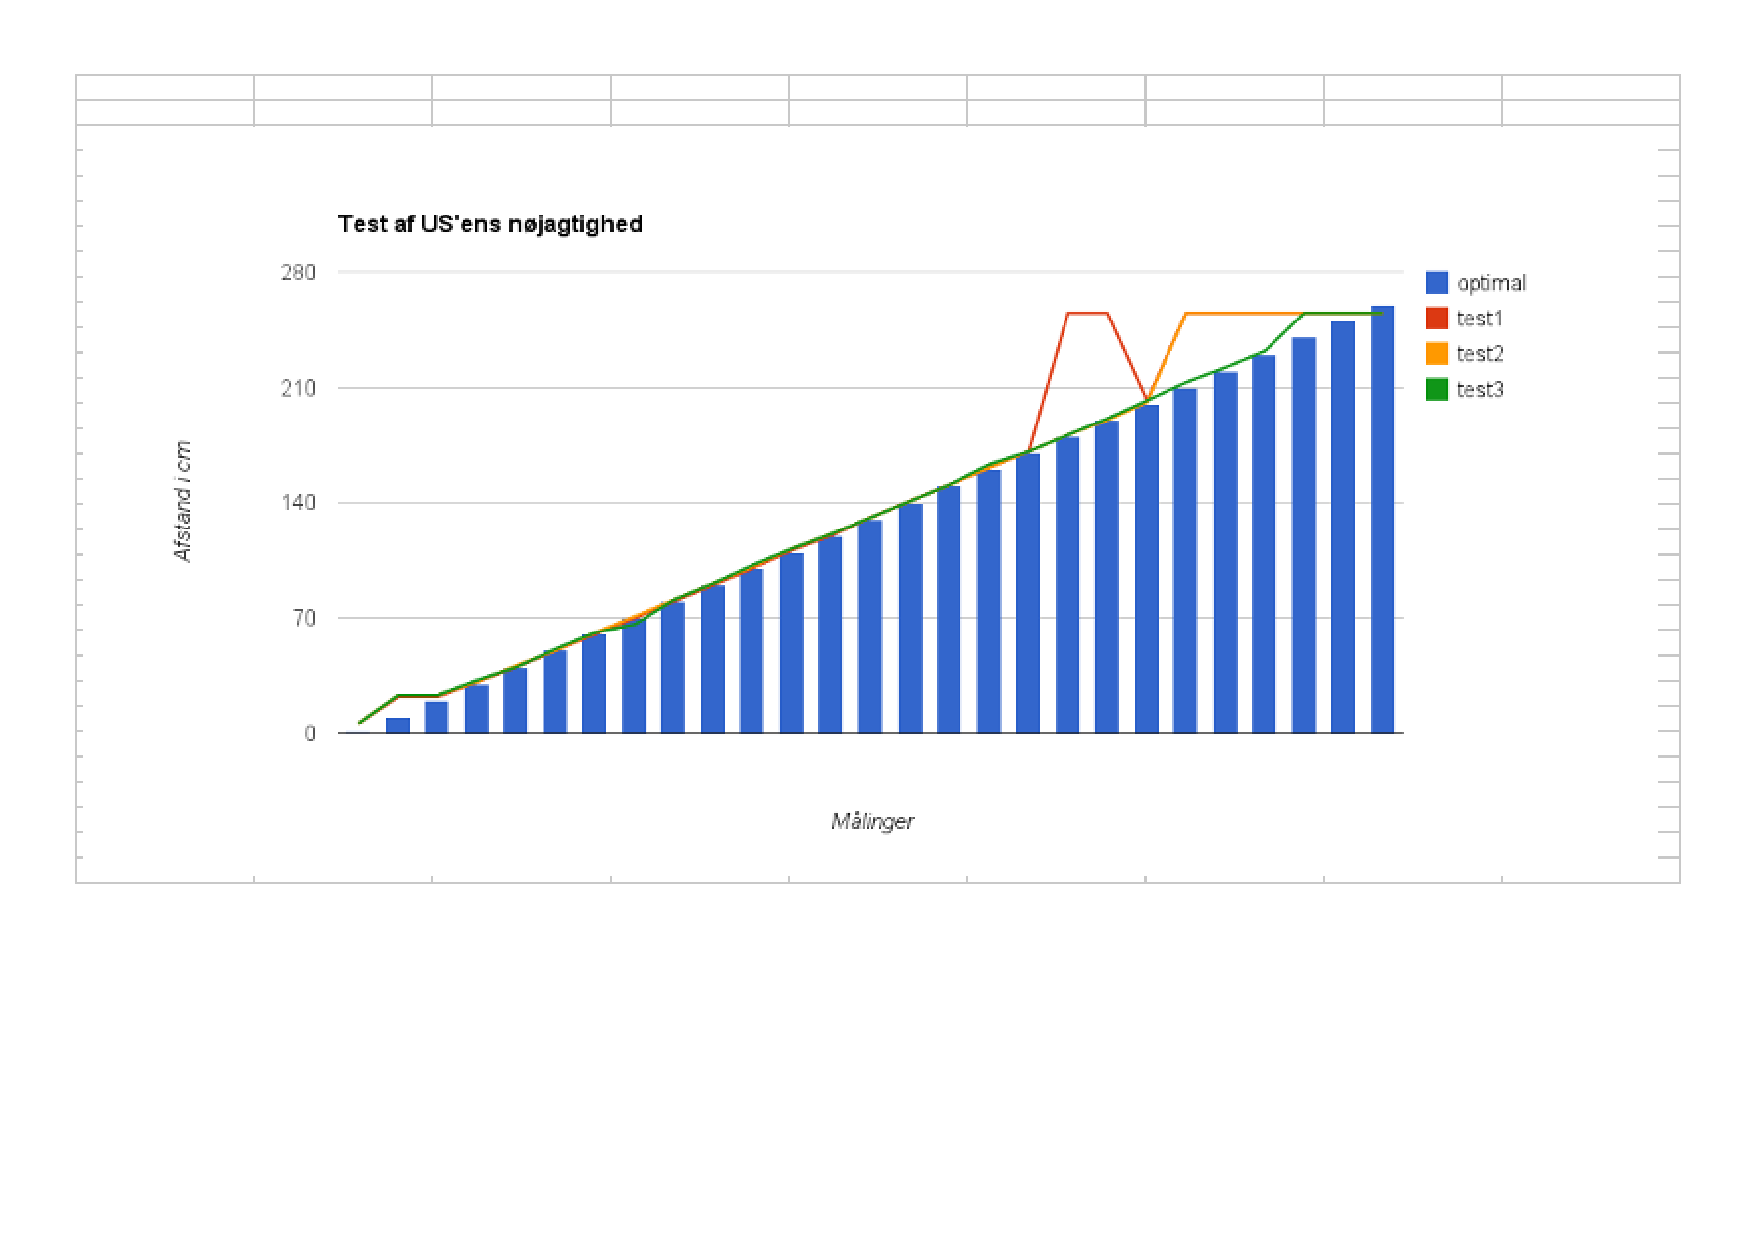
\includegraphics[width=10cm]{us_result_diagram}
\caption{Testresultater: De blå søjler repræsenterer den målte afstand med tommestok, de andre tre viser US'ens testresultater ifht. hianden.}
\label{us_diagram}
\end{figure}


\subsubsection{Infarød Sensor}
Den infarøde afstandssensor(IS) som kan ses på \ref{is} er en afstandssensor med høj præcision og et interval på 10 til 80 cm.

\begin{figure}[h]
\centering
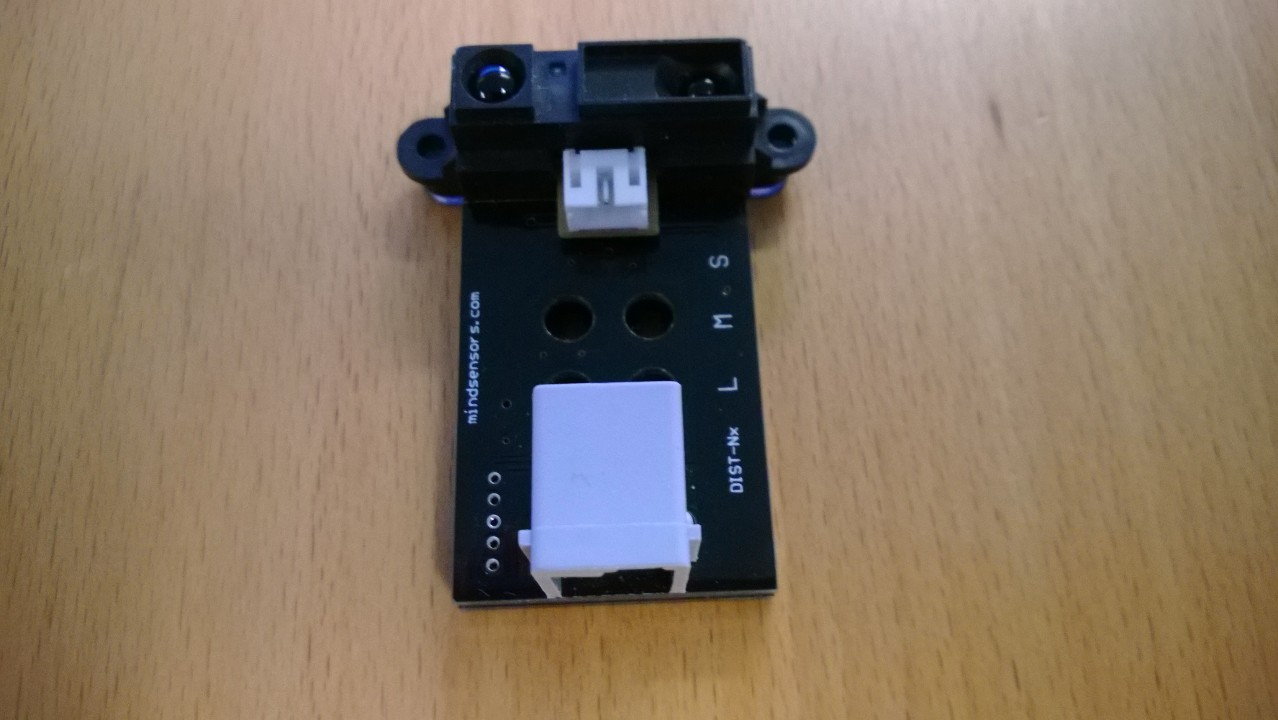
\includegraphics[width=10cm]{is} 	
\caption{High Precision Medium Range Infrared Distance Sensor for NXT (v2)}
\label{is}
\end{figure}

\subsection{Motorer}
Motoren består af en rotationssensor som måler omdrejningerne ved grader, denne har en nøjagtighed på 1 grad. Det er med til at gøre motoren ret præcis. Men denne sensor gør det også muligt at styre ret nøjagtigt hvor meget kraft mortoren skal køre med.
Hvis man kører med flere motorer så har NXT'en indbygget software der gør det muligt at synkronisere disse motorer.
Det er smart hvis den ene motor skulle være stærkere eller svagere end den anden.
\end{document}